\subsection{Technologies}
In order to talk about implementation, first we need to talk about technologies.

\subsubsection{Mobile}
To reach the highest possible amount of users, the application needs to be available in both major mobile operating systems, Android and iOS. Achieving this is possible without two different codebases by using a cross-platform development framework. A lot of alternatives are available, most of them consisting of a web view, providing the ability to use web technologies for development. For scalability and performance reasons, these options are discarded, in favor of a more native, approach possible with React Native or Flutter. These frameworks compile to native code, providing better performance and as a result more room for the app to grow in the future. Finally, between the two, Flutter is the preferred choice as it is a stable release (React Native is still in version 0.61 as of writing this document) and provides a big standard library of UI components, avoiding the need of third party packages and allowing for faster development.

\subsubsection{Back-end server}
The backend will be implemented in Kotlin utilizing the Spring boot framework. Spring is one of the most popular frameworks for the development of web applications. It allows for fast development and easy integration with documentation tools that help speed up the work. Because of its maturity and popularity, there is a great amount of documentation on the framework itself. There are a few alternatives, like Play and Grails, which offer similar functionalities, but Spring has been proven to be the most performant of the three.
The web server will conform to the REST architectural design, providing a REST api, which allows for great flexibility.

\subsubsection{Database}
Due to the need of location searches on the report data, the database management system chosen needs to have support for geospatial queries. Also, there is no need for complex transactions in the system, as updates will be rare and not concurrent, reports are mostly appended to the existing data.
For these reasons, the system chosen is MongoDB, a document-oriented database management system. It provides geospatial queries out of the box, good read and write performance and great scalability with distributed configurations. 

\subsubsection{Image analysis}
A key point of the system is extracting important information from the submitted pictures in the reports. This then implies the necessity to have an image recognition algorithm to detect license plates and cars. Implementing this from scratch would consume too many resources and there is no need to reinvent the wheel, as there are tried and true libraries available. The chosen one is OpenALPR, which provides a public API, but also SDKs for multiple languages, including Java, which can be easily used from Kotlin in the application server.


\subsection{Implementation and integration}
Due to the small size of the development team, communication between team members and change making is not a problem. Because of this, the idea is to progressively integrate every part of the system as soon as they are ready. A component is considered ready once fully implemented and tested.

Both the web server and the mobile application will be developed in parallel, with the mobile app slightly behind in schedule so that any functionality required from the backend is already implemented and tested. This allows the mobile app to safely use the services provided by the backend without failures. In any case, external dependencies in the mobile application will be mocked for implementation and later integrated, which makes the development more predictable and easier for problem detection.

Integration with external services and libraries will take maximum priority, as these are the parts of the system where some modifications might have to be made, and where problems may arise. This is especially true with the photo analyser component, which covers of the core functionalities of the system and has a great amount of uncertainty. 

In terms of the interaction between the backend and the DBMS, this integration will be made from the beginning. Spring boot makes this extremely easy and integration with MongoDB is fully supported.\\

Here the implementation and integration order for the application server is listed along with diagrams showing the dependencies between components:\\

The ReportAnalyzer is prioritized because of its core importance. The ReviewRecruiter is integrated later.
\begin{itemize}
    \item 
    LicensePlateRegistry
    \item 
    PhotoAnalyzer
    \item 
    ReportAnalyzer
\end{itemize}

\begin{figure}[H]
    \centering
    \fbox{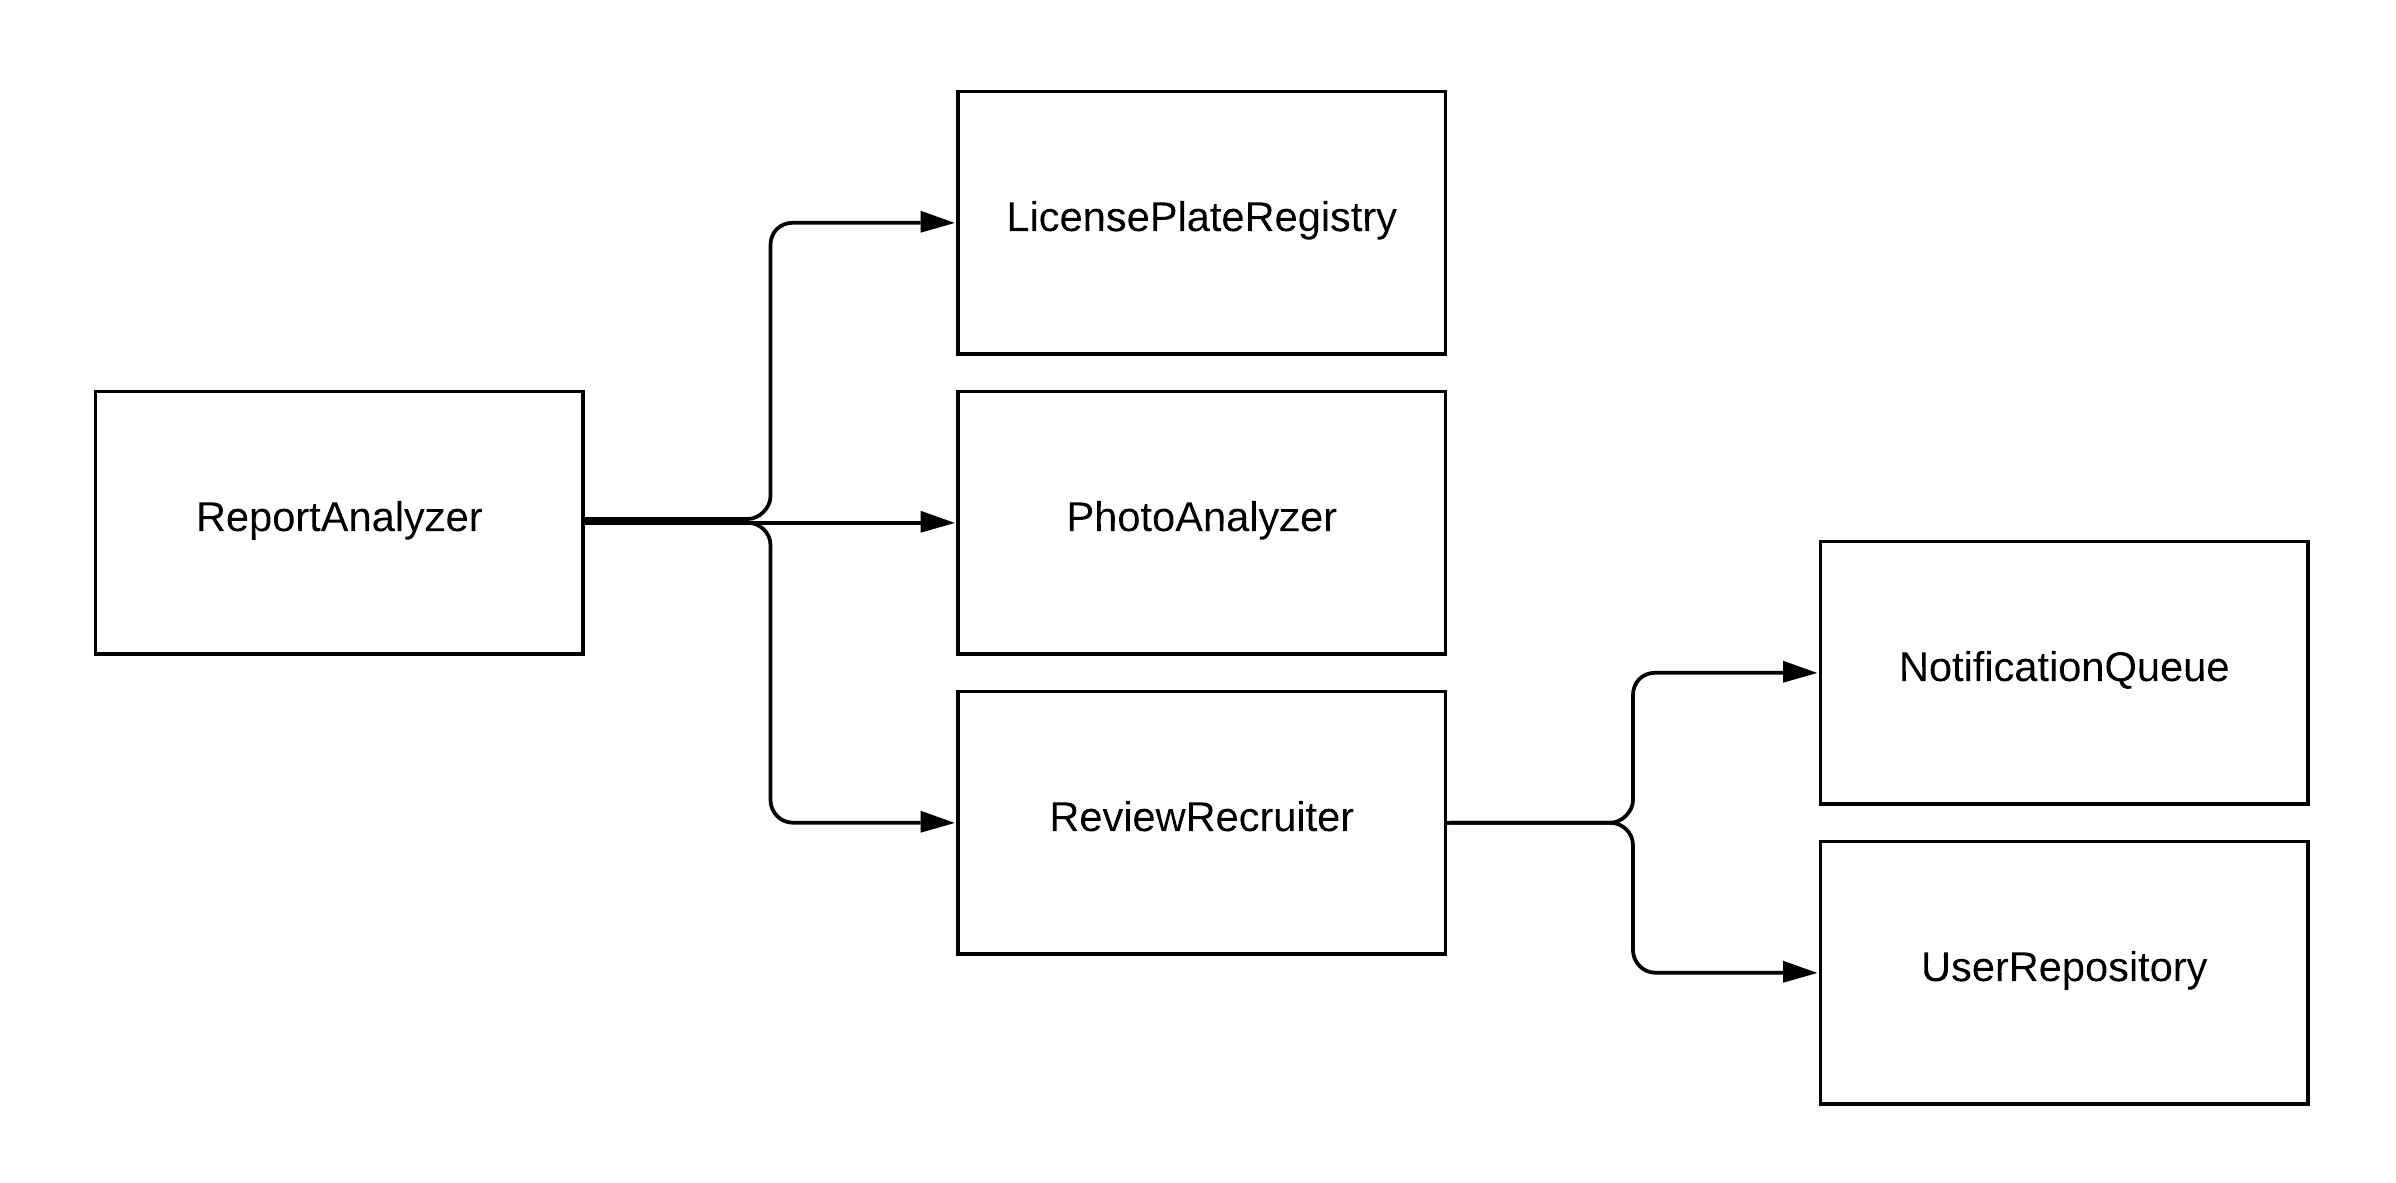
\includegraphics[width=0.95\textwidth]{Images/implementation/ReportAnalyzer-dependencies.png}}
    \caption{\label{fig:ReportAnalyzer-dependencies}ReportAnalyzer dependencies.}
\end{figure}

\begin{itemize}
    \item 
    UserRepository
    \item 
    IdentificationManager
    \item 
    AuthorizationGuard
    \item 
    UserManager
    \item 
    UserService
\end{itemize}

\begin{figure}[H]
    \centering
    \fbox{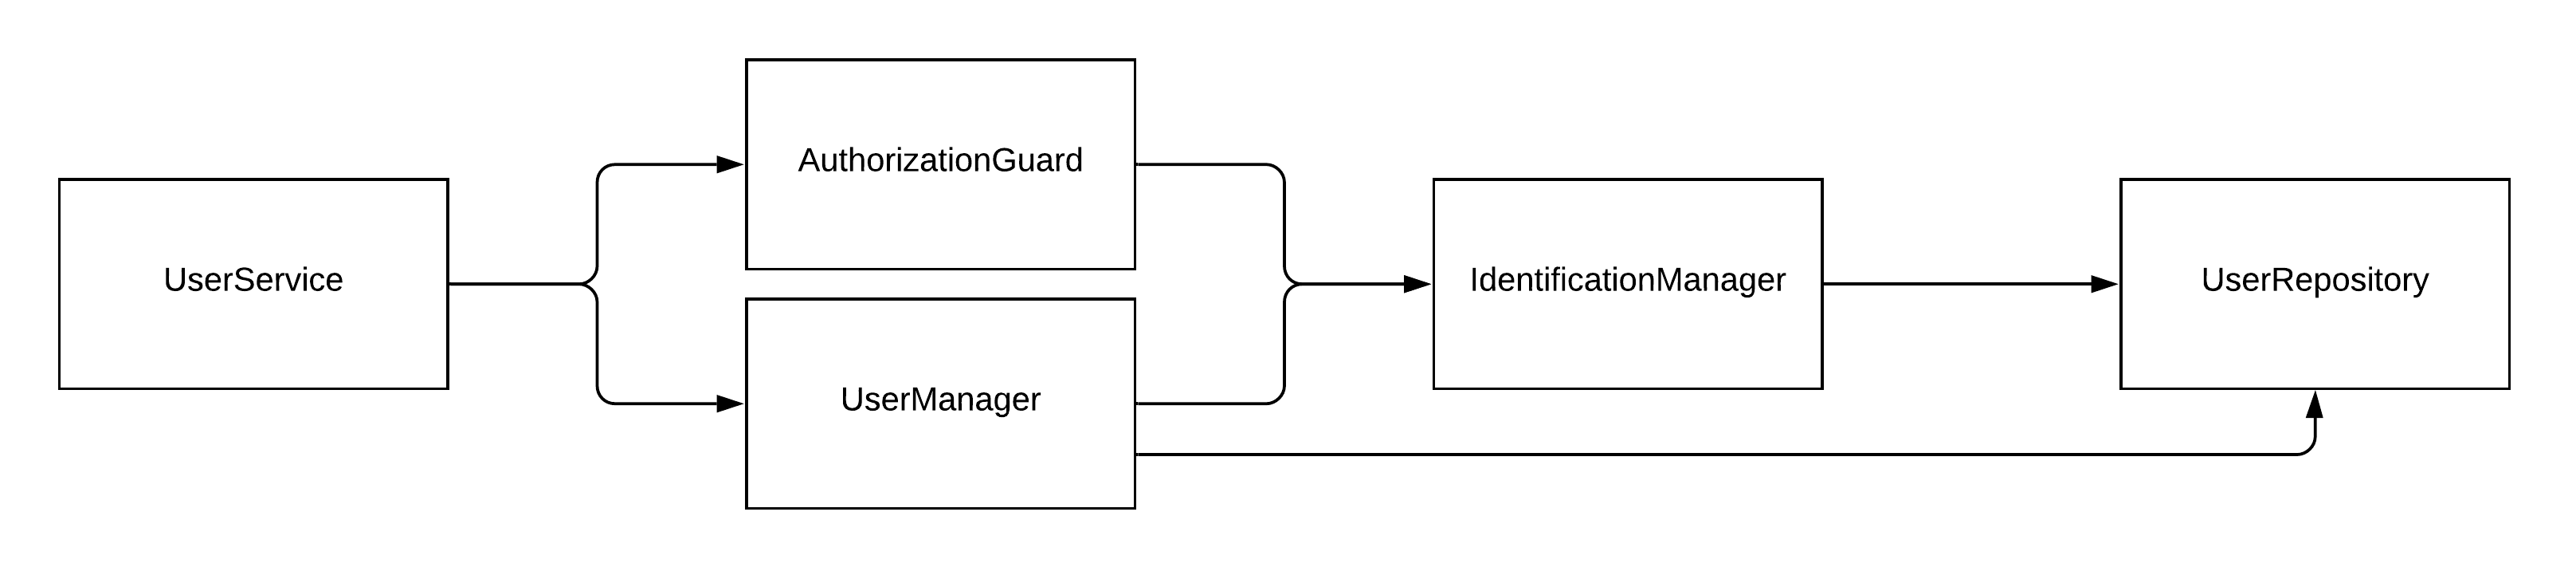
\includegraphics[width=0.95\textwidth]{Images/implementation/UserService-dependencies.png}}
    \caption{\label{fig:UserService-dependencies}UserService dependencies.}
\end{figure}

\begin{itemize}
    \item 
    NotificationQueue
    \item 
    ReviewRecruiter
    \item 
    ReportRepository
    \item 
    TicketingSystem
    \item 
    ReportManager
    \item 
    ReportService
\end{itemize}

\begin{figure}[H]
    \centering
    \fbox{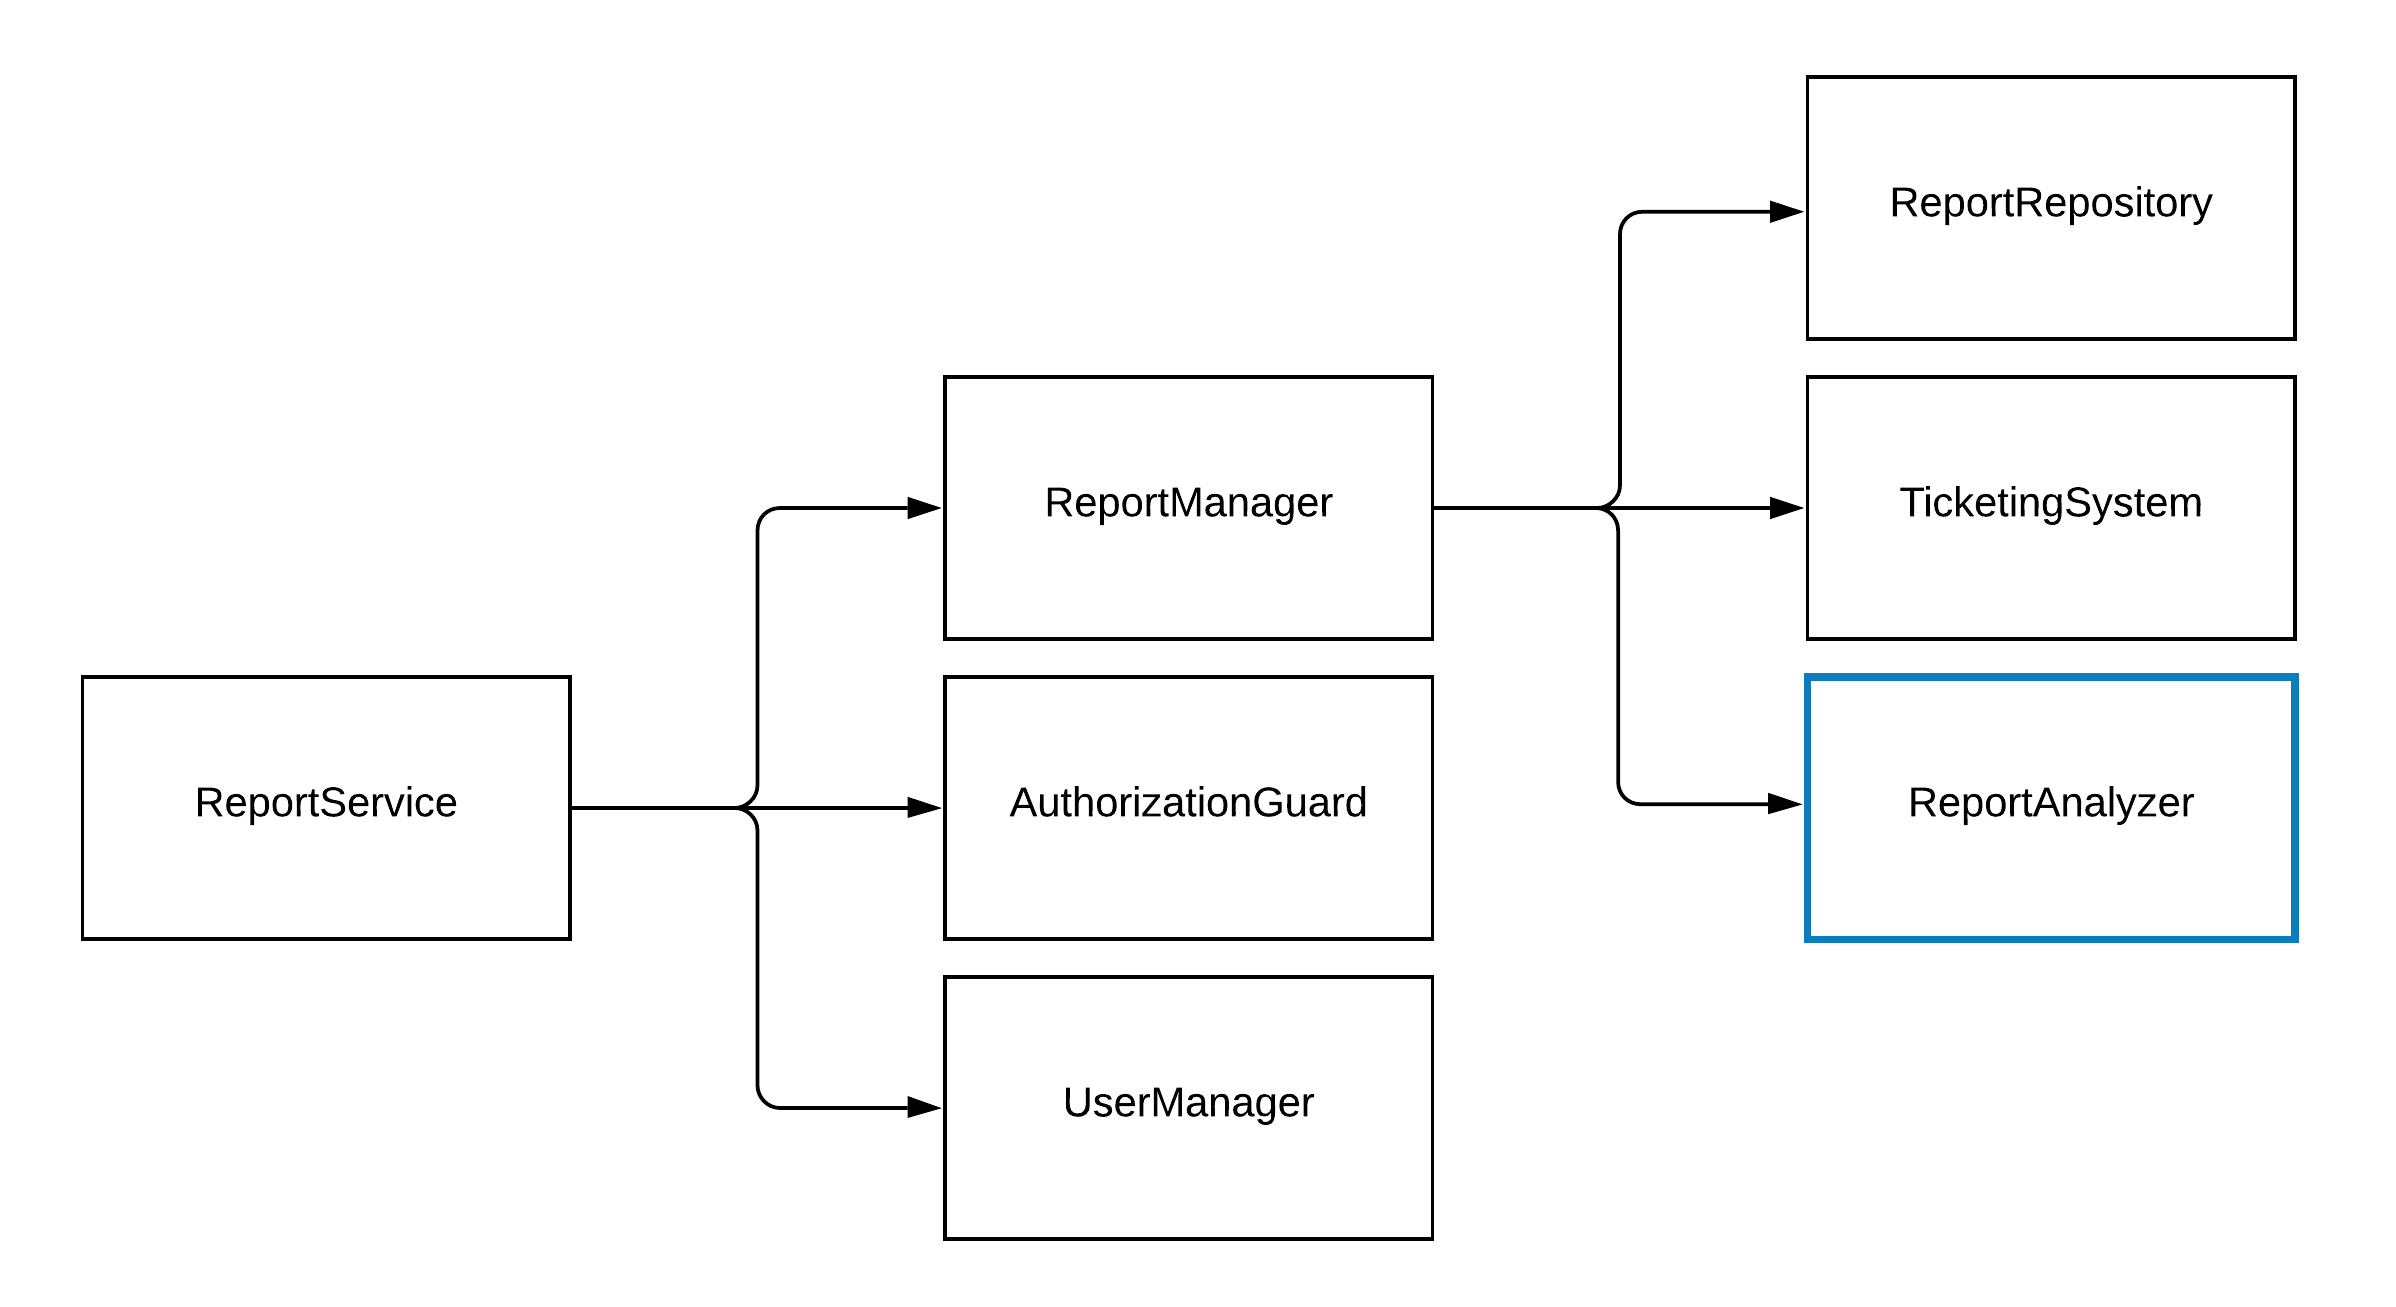
\includegraphics[width=0.95\textwidth]{Images/implementation/ReportService-dependencies.png}}
    \caption{\label{fig:ReportService-dependencies}ReportService dependencies.}
\end{figure}

\begin{itemize}
    \item 
    ReviewRepository
    \item 
    ReviewManager
    \item 
    ReportReviewService
\end{itemize}

\begin{figure}[H]
    \centering
    \fbox{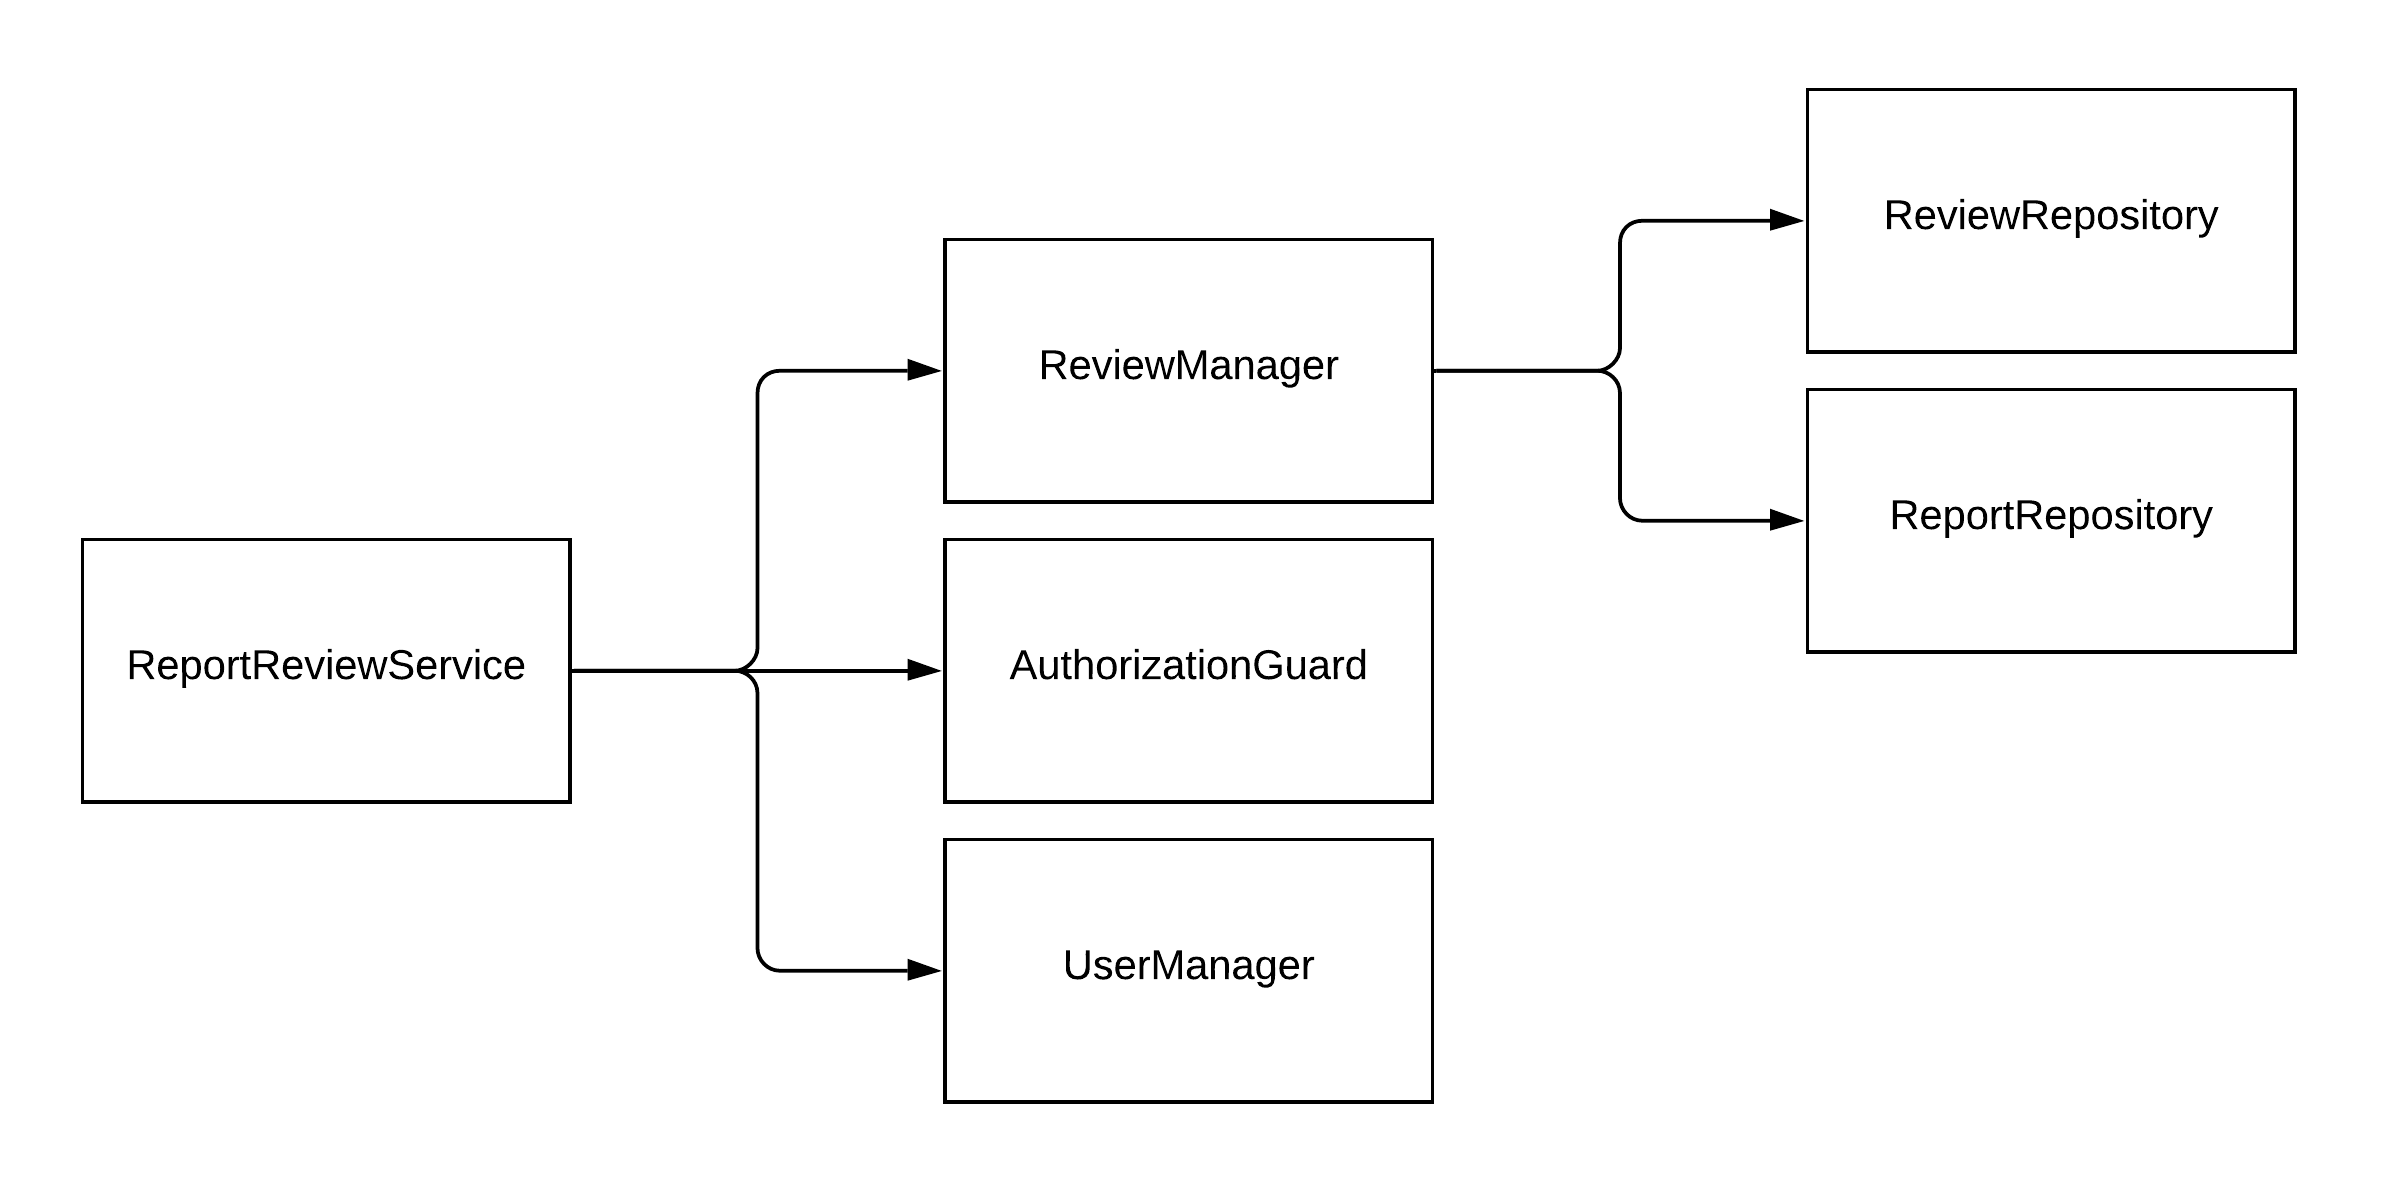
\includegraphics[width=0.95\textwidth]{Images/implementation/ReportReviewService-dependencies.png}}
    \caption{\label{fig:ReportReviewService-dependencies}ReportReviewService dependencies.}
\end{figure}

\begin{itemize}
    \item 
    NotificationService
\end{itemize}

\begin{figure}[H]
    \centering
    \fbox{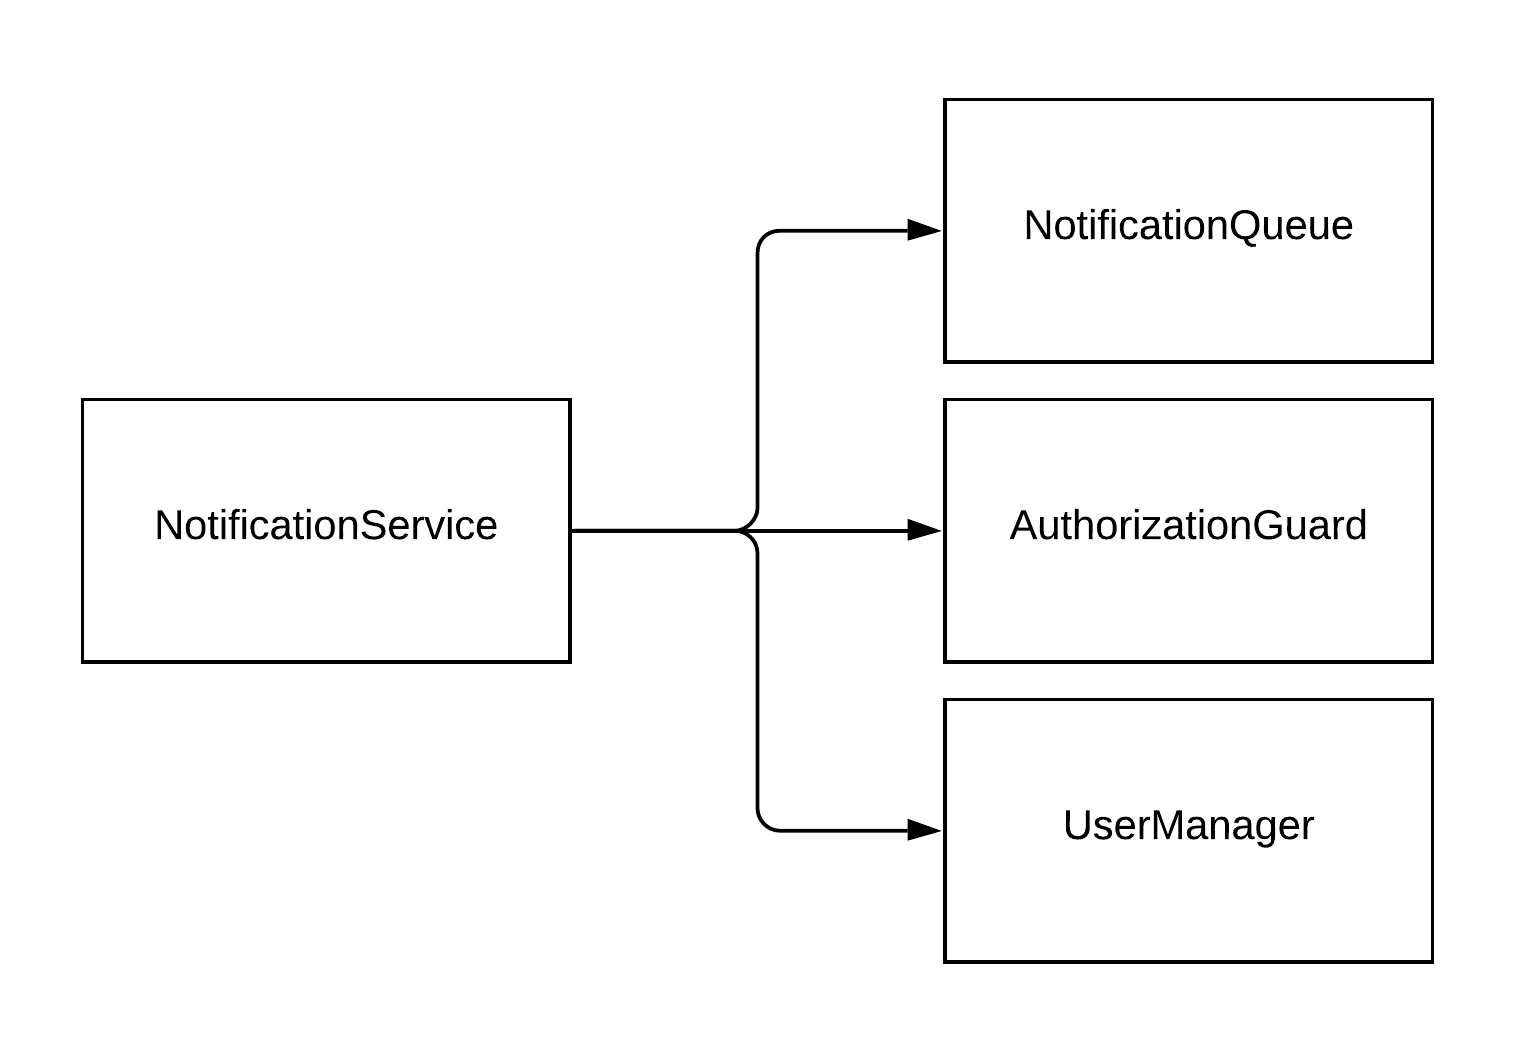
\includegraphics[width=0.65\textwidth]{Images/implementation/NotificationService-dependencies.png}}
    \caption{\label{fig:NotificationService-dependencies}NotificationService dependencies.}
\end{figure}
 
As previously mentioned, the implementation and integration of the mobile app will be done in parallel, in the order listed below. Note that these include both the user interface and the underlying functionalities and integrations:\\

As in the application server, the core of the application is given priority. In this case, it consists of the Report submission and the Report map. Since these components depend on others not yet implemented, they will be mocked until necessary.

\begin{itemize}
    \item 
    Report submission
    \item 
    Report map
\end{itemize}

\begin{figure}[H]
    \centering
    \fbox{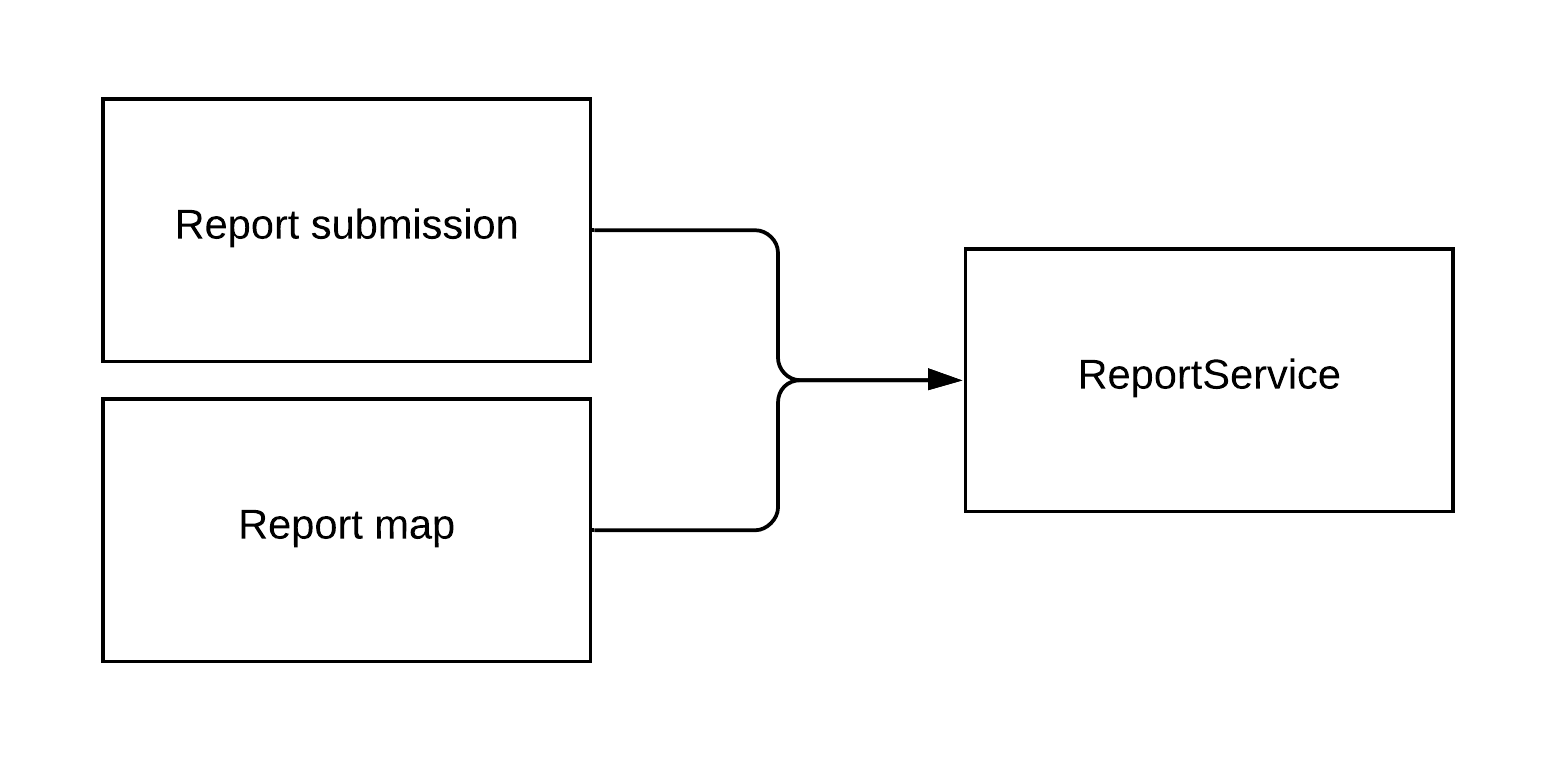
\includegraphics[width=0.65\textwidth]{Images/implementation/reportsubmission-dependencies.png}}
    \caption{\label{fig:reportsubmission-dependencies}Report submission and Report map dependencies.}
\end{figure}

\begin{itemize}
    \item 
    Sign In
    \item 
    Sign Up
    \item 
    Profile
\end{itemize}

\begin{figure}[H]
    \centering
    \fbox{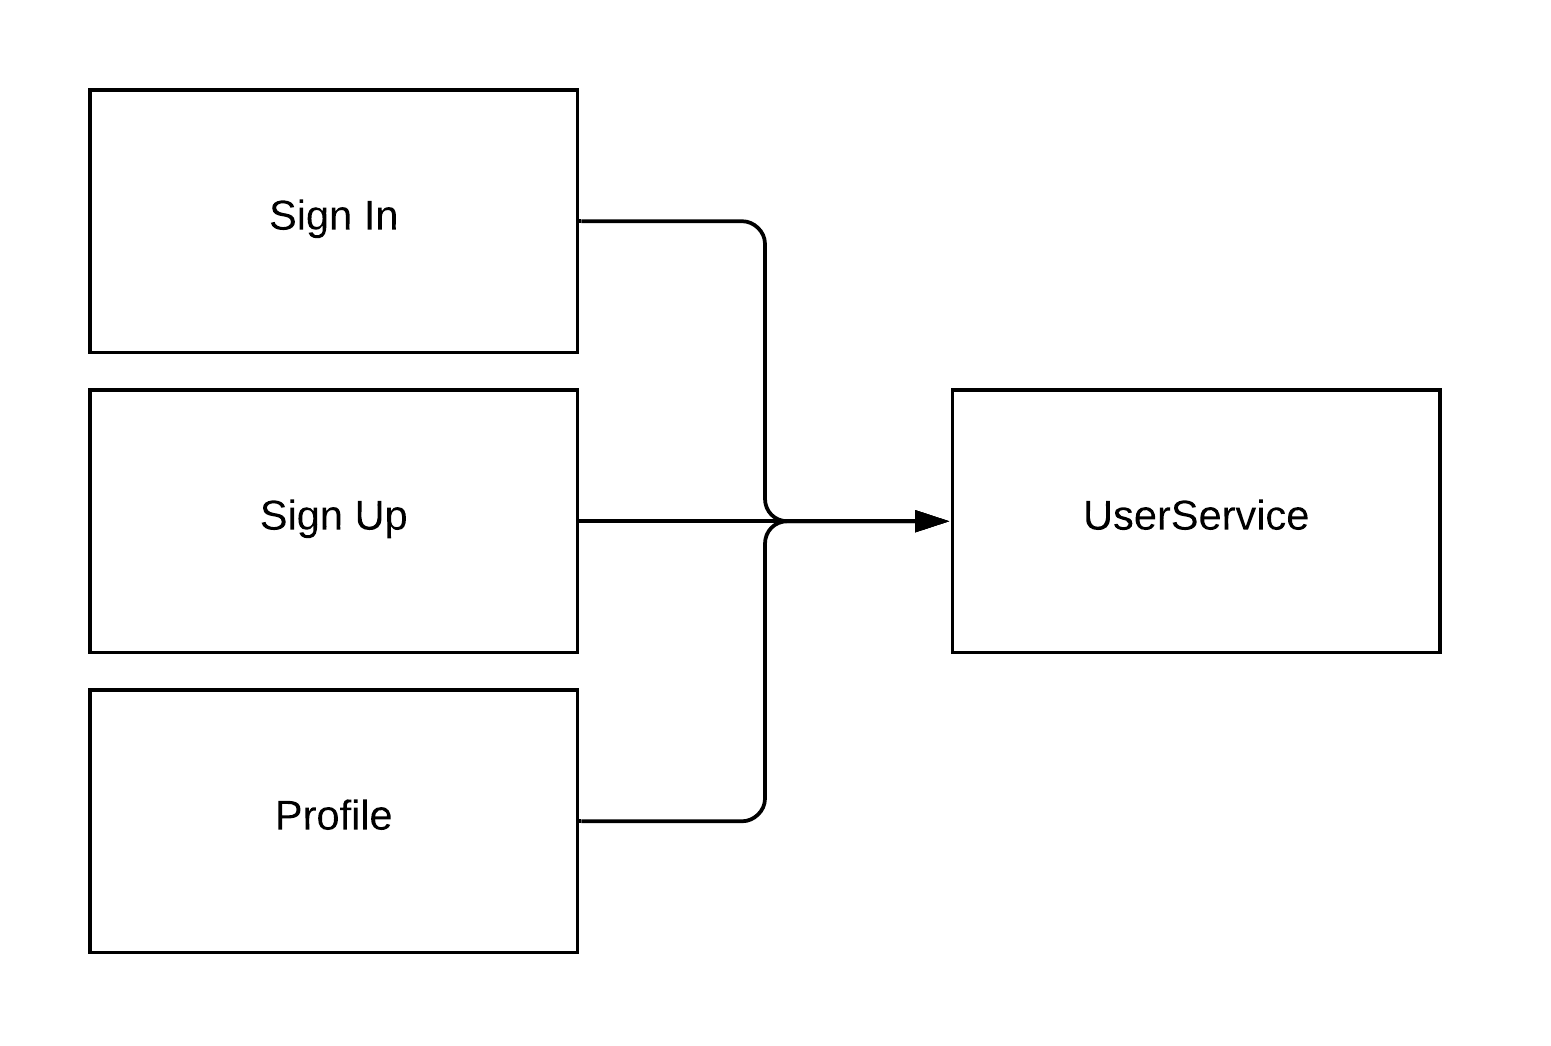
\includegraphics[width=0.65\textwidth]{Images/implementation/signin-dependencies.png}}
    \caption{\label{fig:signin-dependencies}Sign In, Sign Up and Profile dependencies.}
\end{figure}
 
\begin{itemize}
    \item 
    Photo review
\end{itemize}

\begin{figure}[H]
    \centering
    \fbox{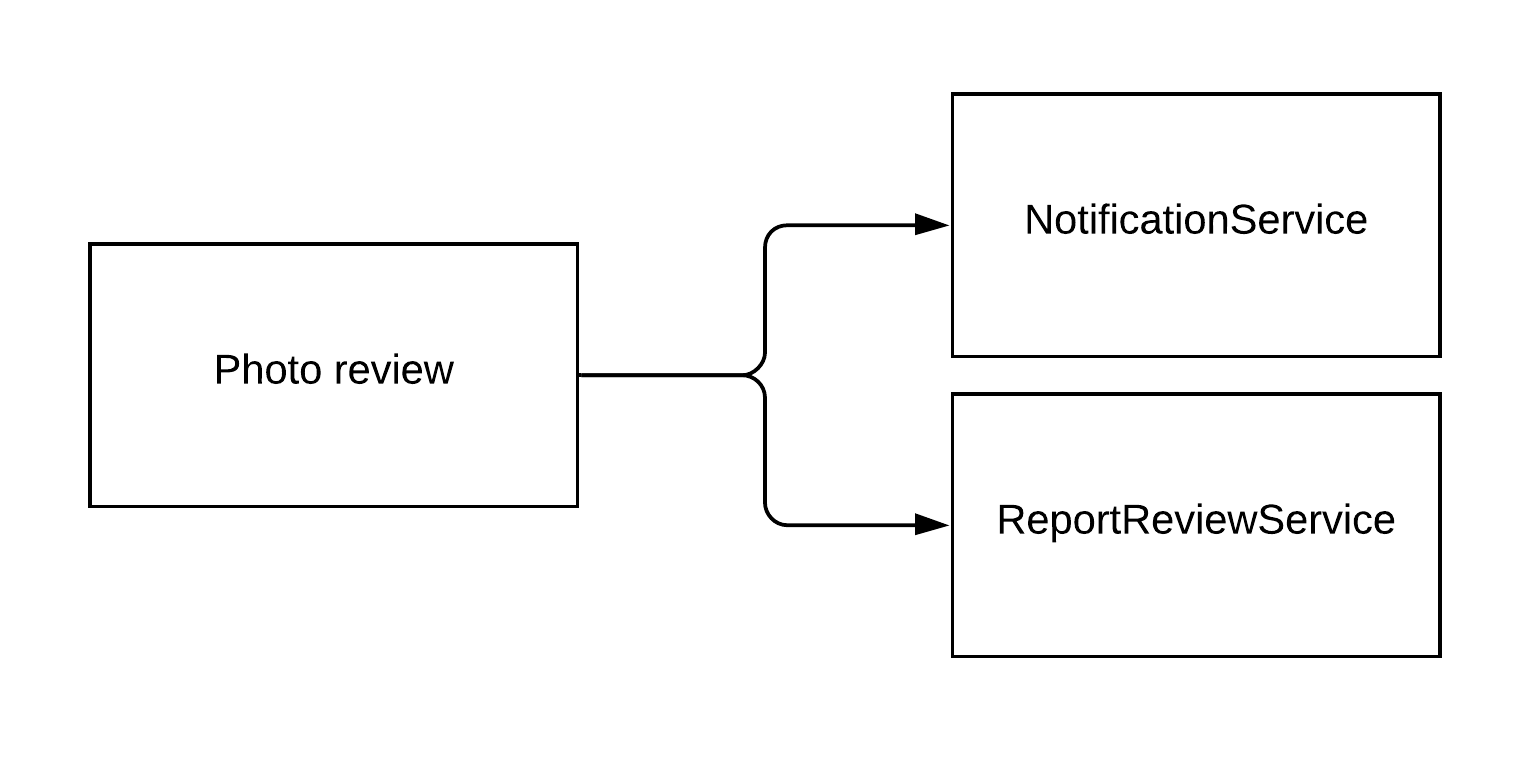
\includegraphics[width=0.65\textwidth]{Images/implementation/photoreview-dependencies.png}}
    \caption{\label{fig:photoreview-dependencies}Photo review dependencies.}
\end{figure}

\begin{itemize}
    \item 
    Home
\end{itemize}

Here screen names are utilized for easy understanding, but note that the screens themselves are not considered components.

\subsection{Testing}
A component is only considered ready for production after its fully tested. There is no established order of testing, this is, the component is continually unit tested while being developed. 
Integration testing will mainly take place in the mobile application, since the external services used in the backend are already tested by their organizations. 
Once a feature is finished in both the mobile app and the backend, e2e tests will be performed to ensure all parts are in working order.

The following technologies will be used for testing:
\begin{itemize}
    \item 
    \textbf{JUnit5} integrated with spring boot for unit testing in the web server.
    \item 
    For mobile, the libraries used will be \textbf{flutter\_test} and \textbf{flutter\_driver} which are designed for UI and E2E testing respectively.
\end{itemize}